\documentclass[a4paper,12pt,english]{article}

\usepackage{amsmath}              % Math mode and text combined
\usepackage[english]{babel}       % Break words in the right place
\usepackage[style=apa]{biblatex}  % References
\usepackage[a4paper, margin={2.5cm}]{geometry} % Default A4 margins
\usepackage{graphicx}             % Images
\usepackage{subcaption}           % Composite images

\addbibresource{bibliography.bib}

\title{Securing Web-Based Electronic Elections
\\
\large Information Security Assignment - Group 1}

\author{Jarne Clauw
    \and
    Tibo De Peuter
    \and
    Robin Meersman
    \and
    Matthias Seghers
    \and
    Emma Vandewalle
    \and
    Tybo Verslype
}

\date{\today}

\begin{document}

\maketitle

\section{Introduction}\label{sec:introduction}

To this day, voting needs to be done at a polling station, where votes are registered with paper ballots or electronic machines. This approach has been around for quite a while, but with the world digitizing fast, the demand arises for an online system where people can cast their votes.

In this report, we propose a web-based system as an alternative to physical voting. We first explore the requirements for fair elections, and how they are reflected in our model. We then continue with the potential attacks, along with the countermeasures to prevent them. Finally, we look at the limitations and vulnerabilities of our designed system.

\section{Requirements for fair elections}\label{sec:requirements}

Traditional physical elections are built on a foundation of fairness and transparency. As we examine the development of web-based voting, it is essential to establish these fundamental requirements and build from there for any electronic voting system.

\subsection{Physical voting}\label{sec:requirements-physical}

First, let us consider the essential criteria to ensure free and fair elections. These include ensuring citizens have unrestricted access to voter registration processes, casting their ballots with undue burden or restrictions, and providing reasonable accommodations for individuals with disabilities or health conditions that may impact their ability to vote. Furthermore, it should be ensured that elections are conducted independently of government interference, vote counting is accurate and reliable, and citizens have access to readily available, unbiased information to inform their decisions.~(\cite{european-liberties-platform-2021})

\subsection{From electronic to online voting}\label{sec:requirements-online}

Electronic voting systems have been introduced over the years as an alternative to traditional paper ballots, allowing voters to cast their votes using machines or digital platforms. These systems have faced criticism for lacking verifiability properties, making it difficult to ensure that the voting process has not been tampered with. The concerns surrounding the integrity of electronic voting systems underscore the need for robust security measures.~(\cite{cryptoeprint:2016/287})

More recently, there has been an increasing interest in online voting systems that are secure and trustworthy.~(\cite{10.1145/2660267.2660315},~\cite{10.1007/978-3-030-51280-4_3},~\cite{263858},~\cite{halderman2015new}) Such systems allow the user to cast their vote remotely, using a web-based system. This shift towards online voting introduces several additional requirements for information security. In the data security community, five fundamental requirements are widely recognized: data confidentiality, data integrity, availability, authenticity, and auditability, also known as non-repudiation or accountability. While these requirements are well-established, their application in the context of online voting may require their own interpretation. We will delve into these cases in the following paragraphs.~(\cite{gerber-2001})

\subsection{Traditional requirements in context}\label{sec:requirements-context}

\textbf{Authentication} and \textbf{authorization} are fundamental concepts in information security: the system must verify the identity of the user (authentication) and ensure that they are eligible to participate in the voting process (authorization). To meet these requirements, the system should be designed to prevent adversaries from simulating a legitimate voter during registration. Voters should also not be able to cast their vote multiple times, as each vote should only count once.~(\cite{NAP25120})

In the context of information security, \textbf{data integrity} or verifiability ensures that transmitted data remains unchanged and accurate from sender to receiver. In the specific case of web-based voting, this property includes accuracy, as well as ensuring that the final tally is correct. This means that each voter should be able to verify that their vote accurately was recorded, that all votes were correctly counted in the final tally, and that only valid votes were counted. This property is often referred to as the ``cast-as-intended'' principle.~(\cite{4531164})

Voting systems must satisfy the \textbf{confidentiality} requirement, ensuring that voters’ choices remain secret throughout the entire voting process. This includes providing voter anonymity, meaning that the system never reveals how an individual voted, both during submission and after the voting period is over. However, in the context of remote voting, anonymity alone may be considered insufficient, as the lack of a secure and regulated environment, such as the voting booths with official regulators nearby in the case of ballot voting, can make voters vulnerable to coercion. In such cases, it is essential to enable voters to appear as though they are complying with demands from coercers while still maintaining the secrecy of their vote.~(\cite{4531164})

\textbf{Non-repudiation} refers to the inability of the source of information to deny its origin or ownership. In the context of voting, this requirement is crucial, as it ensures that each vote can be traced back to their original voter. Without non-repudiation, votes could potentially be generated fraudulently, violating the integrity of the voting process and undermining authentication and authorization mechanisms.~(\cite{yousuf-2011})

Finally, a reliable voting system must also prioritize \textbf{availability}, ensuring that voters can cast their votes without interruption. This requirement should be considered independently of the fact that this is a voting system, as existing techniques can be leveraged to achieve high availability. Our prototype will therefore not focus on developing novel solutions for this requirement.~(\cite{challenger1998scalable},~\cite{baker2011megastore})

\section{A design for secure web-based elections}\label{sec:design}

To ensure fair and secure elections, as described in the previous section, several factors must be considered. Our online voting system consists of four essential components: a client, an intermediary server, an authentication server, and a backend server. This architecture is illustrated in Figure~\ref{fig:schematic}, providing an overview of the system's design.

\begin{figure}
    \centering
    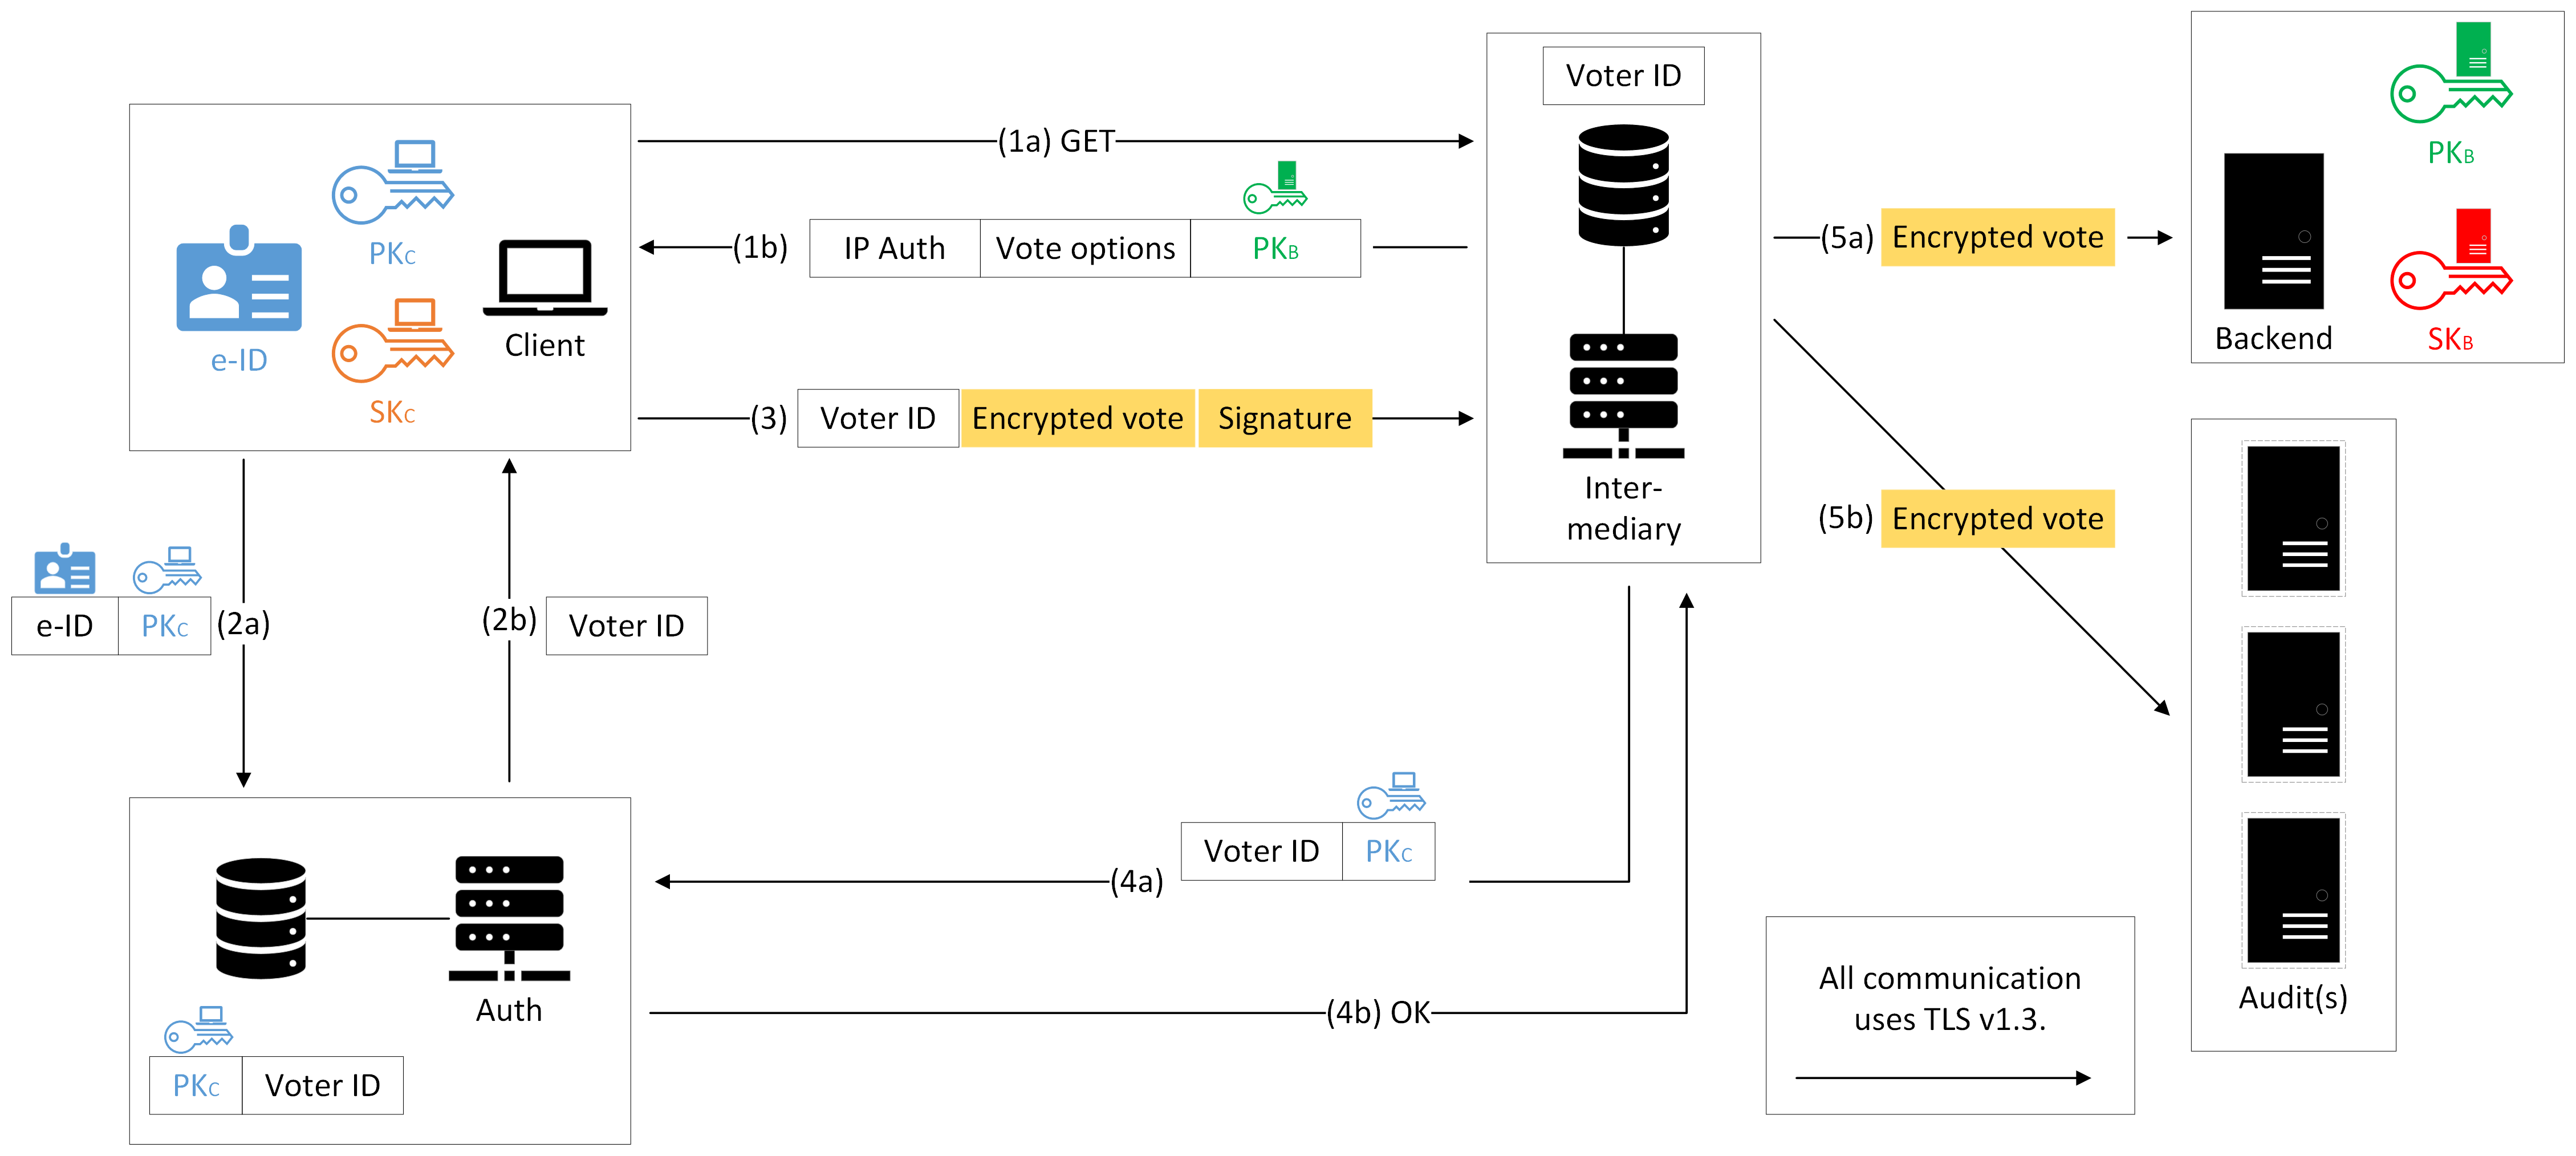
\includegraphics[width=\textwidth]{Schematic}
    \caption{The web-based model}\label{fig:schematic}
\end{figure}

\subsection{Availability}\label{sec:design-availability}

From the perspective of a voter, the first step is to search for the election website. However, many people will follow the first link they find without verifying its authenticity. Therefore, it is crucial to provide clear instructions on how to access the legitimate voting website. One approach is to utilize the existing services of ``Mijn Burgerprofiel'', a personal online hub that consolidates all official government information and administrative data, that every Belgian citizen possesses, and make the link to the voting website readily available. This method also enhances security by limiting the spread of information about the election website to unauthorized parties.

Furthermore, a time-slot allocation system can be implemented to prevent a surge in requests and ensure availability. Each citizen would receive a specific time window during which they are allowed to cast their vote. This method mitigates the risk of congestion and ensures a smoother online voting experience.

\subsection{Authentication and authorization}\label{sec:design-auth}

When the voter accesses the page during their given time slot, the next step is to verify their identity. Before establishing a connection with the authentication server, additional information is required. That’s why the client first communicates with the intermediary server, whose IP-address is stored in a configuration file. The intermediary server then sends the IP-address of the authentication server, along with the public key of the backend server and a list of available voting options. This data is sent over a TLS connection to secure communication between the client and intermediary server. With this information, the user can authenticate themselves using their e-ID credentials, which confirms their identity. The process of authenticating users is discussed in more detail at the end of this section (\ref{sec:design-algos}). The authentication server will authorize the user if they are allowed to cast a vote. Behind the scenes, an asymmetric keypair is generated as part of this process. The public key of the generated keypair is sent to the authentication server, who will then store it in a table, along with a generated voter ID. The authentication server returns this voter ID to the client, effectively making sure that no other user can vote in place of the verified user, all while disclosing the actual identity of the user.

\subsection{Casting the vote}\label{sec:design-casting}

After successful verification, the user can cast their vote from among the previously received list of available voting options. Notably, each user gets the same set of options, which means that simply encrypting only the chosen option(s) and sending it to the backend server is insufficient, as multiple users would produce identical outcomes when they pick the same option. To solve this issue, a nonce, generated using the current timestamp and the fingerprint of the client's public key, is appended to the vote message. The backend server's public key is then used to encrypt both the vote and nonce value together. To ensure the authenticity of the vote, the user's private key is used to sign the output along with their voter ID. The result is sent to the intermediary server using TLS.

Formally, these steps can be written down as formula~\ref{formula:signed_vote}.

\begin{align}
    \text{Signed vote} &:= \text{Sig}_{SK_C}(\text{Enc}_{PK_B}(\text{vote}, \text{salt}), \text{voter ID})\label{formula:signed_vote}
\end{align}

\begin{figure}
    \centering
    \begin{subfigure}{0.48\textwidth}
        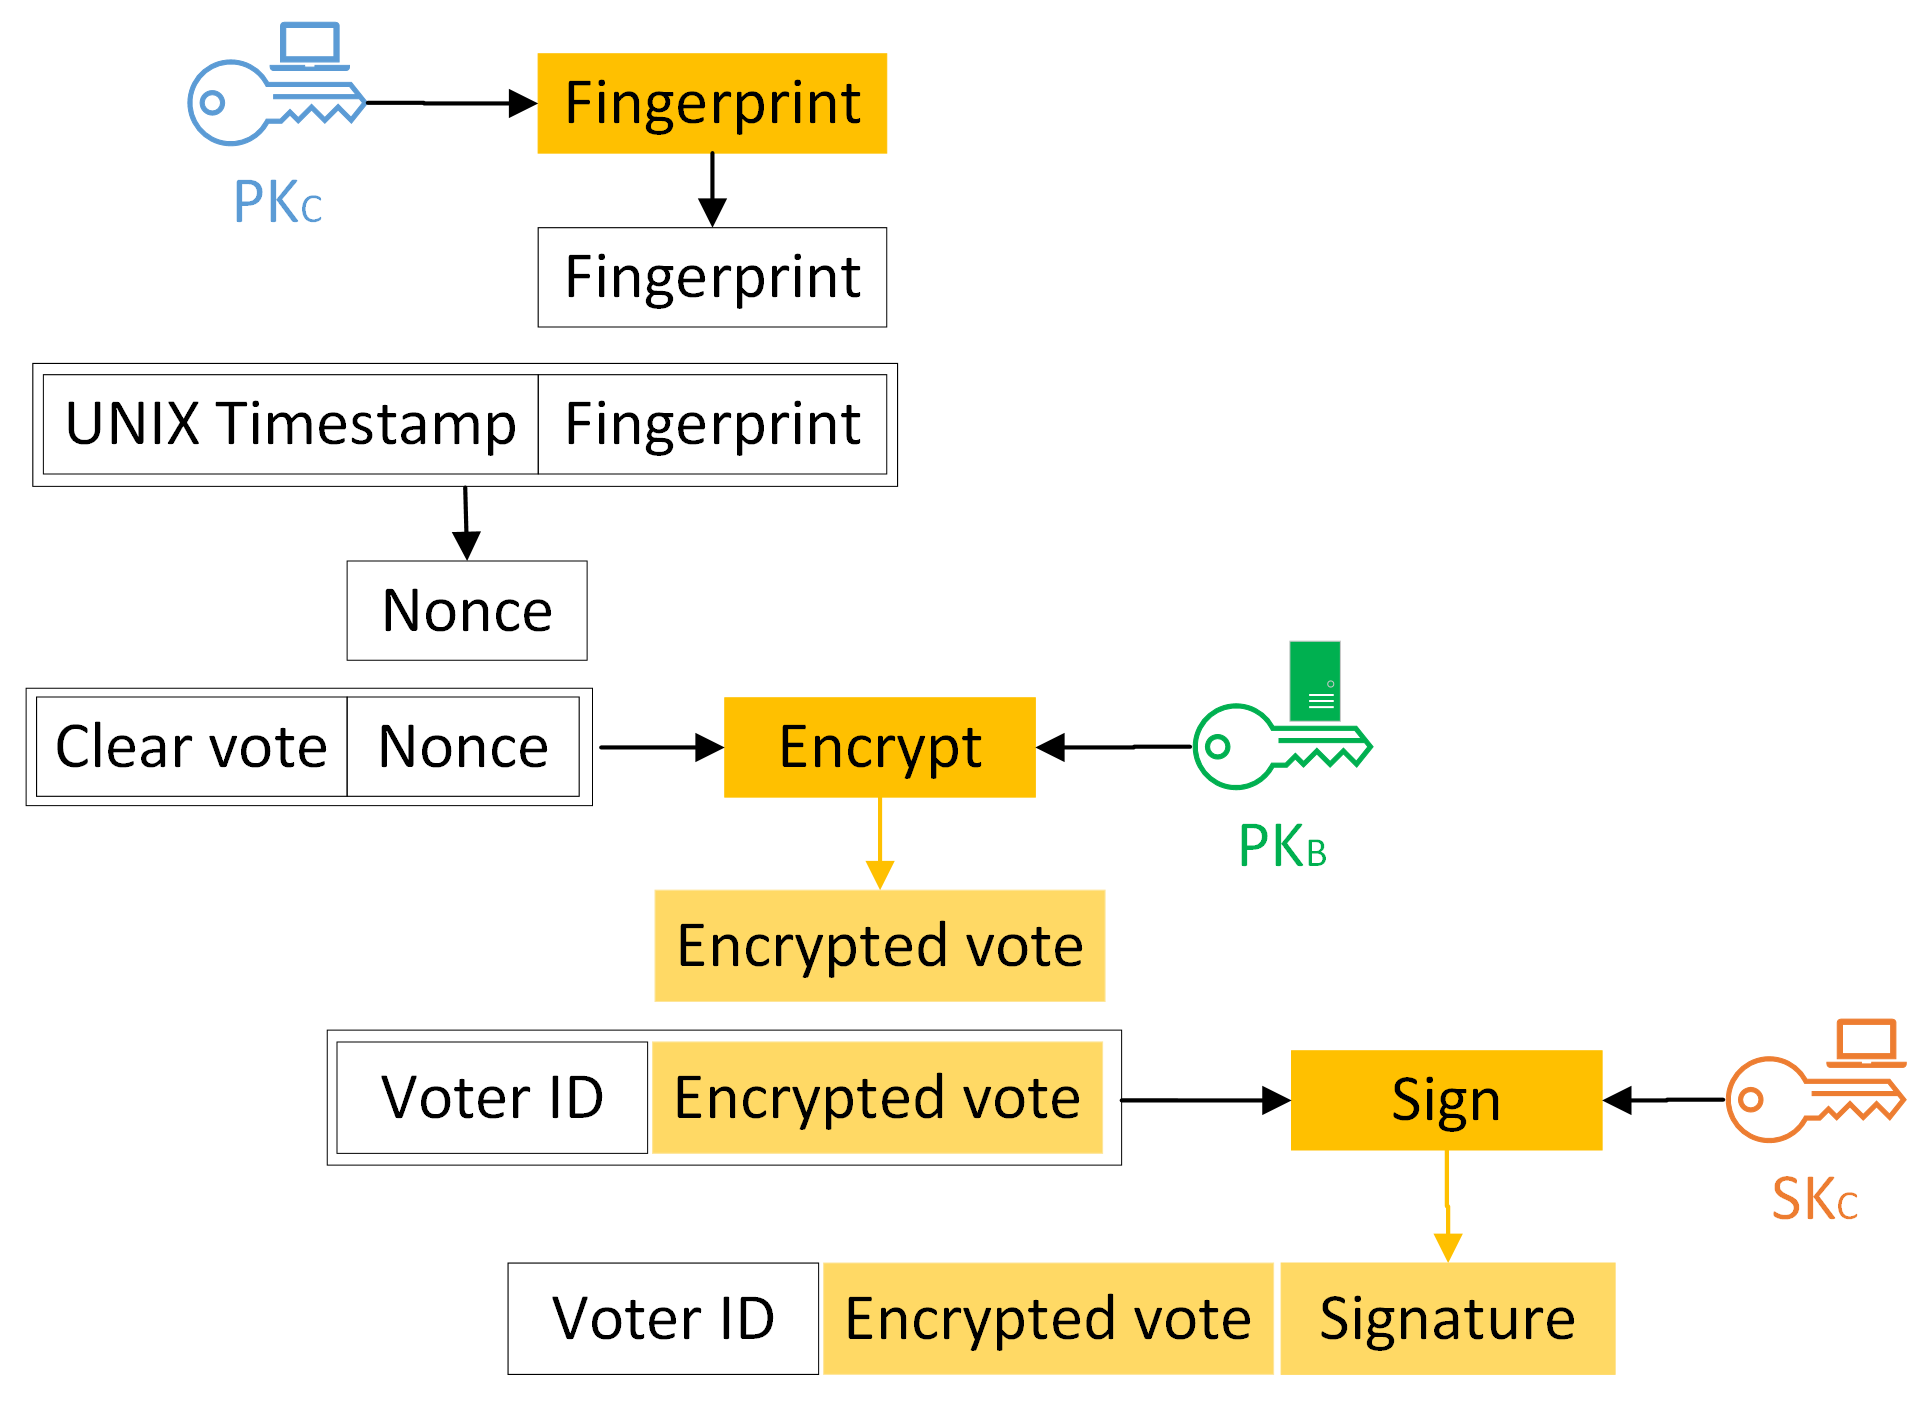
\includegraphics[width=\textwidth]{Client_Protocol}
        \caption{Client protocol}\label{fig:client}
    \end{subfigure}
    \begin{subfigure}{0.48\textwidth}
        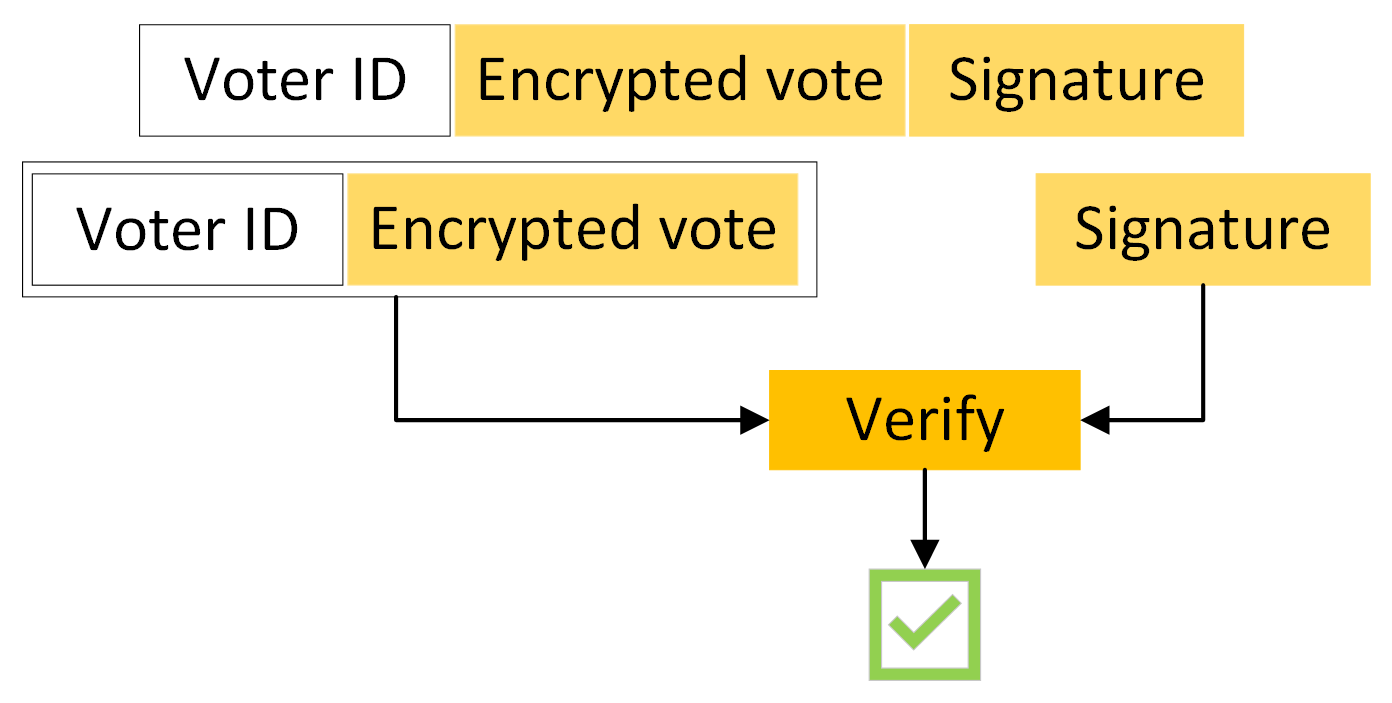
\includegraphics[width=\textwidth]{Intermediary_Protocol}
        \caption{Intermediary protocol}\label{fig:intermediary}
    \end{subfigure}
    \caption{Protocols in the web-based model}
\end{figure}

To maximize the ease of use for the user, the client must only execute the steps described above. What happens next is without the knowledge of the client.

\subsection{Verifying the vote}\label{sec:design-verifying}

Before forwarding each vote to the backend server, the intermediary server verifies its authenticity. This process involves validating the vote using the received signature and the public key of the client. If verification was successful, the intermediary server queries the authentication server to confirm whether the combination of the voter ID and key used for signing is stored in its database. If a match is found, it is confirmed that the voter ID was previously generated for that client and stored in the authentication server database, ensuring that the vote is from a legitimate user. The intermediary server can now proceed to forward it to the backend server. However, it will first transform the vote data, as described next.

\subsection{Forwarding the vote}\label{sec:design-forwarding}

To ensure data confidentiality, in this context called vote secrecy, our architecture employs a mechanism that maintains the separation of votes from user information. The vote is encrypted at the client and cannot be recovered by anyone other than a backend server. Before sending the vote to the backend server, the intermediary server removes the user identifying information from the original message, thereby protecting their privacy.

The intermediary server also accommodates an essential feature: storing every voter ID in its database after a user submits their vote. This prevents multiple voting attempts. While the architecture permits multiple votes from the user's perspective, it will discard packets once it detects that a user has already voted. This mild measure is designed to protect users from being forced to vote again, as the forced second vote will not be registered again, although it may not be foolproof.

Finally, the intermediary server should transmit the received packet from the authentication server to all the backend servers. The servers can then decrypt the packet using their private key and securely store the decrypted vote and nonce in its database without any knowledge of who cast it. If the backend servers encounter the same nonce, they drop that vote. This makes sure the vote is never used multiple times.

The multiple backend servers are in place to guarantee that votes are accurately counted in case of a security breach in the backend server. With this last step complete, the process of casting a secure vote is finished.

\subsection{Algorithms and technical details}\label{sec:design-algos}

Several technical details of the architecture will be discussed here.

% PARAGRAPH Authentication services

The authentication server can authenticate users by integrating with the existing infrastructure of the Belgian government, more specifically CSAM, which allows users to log in using their e-ID and a smart card reader or itsme®. We assume this provides sufficient authentication in our context.

% PARAGRAPH Generation of voter IDs, without clashes

To choose an anonymous voter ID, it's important to consider that all IDs should be unique. A simple approach would be to use an incrementing ID starting from zero. However, when using external authentication services, it’s reasonable to assume that their implementation is sufficient to ensure unique voter IDs.

% PARAGRAPH Algorithms for key generation

In our implementation, encrypting and signing will depend on GnuPG. Keypairs will be generated using RSA 2048. Those are strong enough to be considered safe, without requiring too much computation. One could suggest RSA 4096, but this just needs more compute while the extra security isn’t needed in this case. Signatures will be created using SHA256. In fact, these are common options when using GnuPG.

% PARAGRAPH TLS

All communication between entities should be confidential and data integrity should be ensured. We would therefore use TLS on every link in the architecture. Specifically, we would utilize TLS version 1.3 with standard parameters.

\section{Attacks and their countermeasures}\label{sec:attacks}

In this section, we will explore some common attacks and how our architecture mitigates these attacks. We assume a basic understanding of well-known attacks.

\subsection{Eavesdropping}\label{sec:attack-eavesdropping}

Our architecture provides countermeasures against eavesdropping on the network. All connections are secured by TLS 1.3 encryption, while the voting data being transmitted is additionally encrypted with the public key of the backend server. Furthermore, the intermediary server removes any identifying information from the transmitted encrypted voting data, making eavesdropping on the link between the intermediary server and backend server ineffective.

\subsection{Traffic analysis}\label{sec:attack-traffic}

Traffic analysis is insufficient to reveal valuable information. While it may be possible to figure out who cast their vote based on the network traffic between the client and the intermediary server, the actual voting data remains confidential.

Additionally, it could be possible to find the IP addresses of the backend server or the authentication server by analyzing the traffic between those servers and the intermediary server. Fortunately, these servers have their own (services and) security systems in place to protect them.

Optionally, we recommend using Privacy-Enhanced Technologies (PETs) to allow for Traffic-flow confidentiality and further enhance security.

\subsection{Impersonation}\label{sec:attack-impersonation}

Users must authenticate using their e-ID or the itsme® service. In both cases, our architecture relies on the robustness of these respective authentication services. All packets received at the intermediary server are digitally signed by the authenticated user and verified.

Potential weaknesses still exist and will be discussed in Section~\ref{sec:limit-impersonation}.

\subsection{Replay}\label{sec:attack-replay}

We employ a mechanism that allows users to vote only once and ignores subsequent attempts. Replaying packets to the intermediary server will be discarded, effectively increasing network traffic without compromising the integrity of the data.

Replaying packets to the backend server are countered by using TLS 1.3 and the nonce added inside the encrypted vote.

\subsection{Distributed Denial of Service (DDoS)}\label{sec:attack-ddos}

Different systems can be put into place to mitigate the risk of DDoS attacks. These systems must be set up for both the intermediary and the backend servers. Apart from using high bandwidth servers we could use filtering and limiting techniques, caching, and other established solutions. While this aspect is more related to server maintenance than a direct security concern, it is crucial to ensure the availability of our system using existing techniques independently of the context of web-based voting.

\subsection{Sybil attack}\label{sec:attack-sybil}

The Sybil attack, as described on~\cite{wikipedia-contributors-2023}, involves creating many pseudo-identities to manipulate the reputation system. Our architecture is designed to mitigate this type of attack by requiring each user's identity to be linked to an official, registered ID-card.

\section{Limitations and vulnerabilities}\label{sec:limitations}

The system we have described to make online voting possible does not go without its limitations and vulnerabilities.

\subsection{Compromised client}\label{sec:limit-client}

Since the client is the entry-point for a user to vote. If an attacker gets access to the client, it can read the identity of the user and the vote they cast. Then the attacker can choose which votes he sends further down the model.

This problem could be solved by first making a connection with the authentication server and receiving a public key which is tied to the user's identity. With the help of a certificate authority the user can get access to the right public key of the client and send the vote securely through public key encryption.

\subsection{Compromised authentication server}\label{sec:limit-auth}

The authentication server keeps a record of the voter’s id and public key. If an attacker gets access to the authentication server, he could add new records with a chosen voter id and public key. This makes it possible for the attacker to vote multiple times and thus manipulate the voting process.

This is not a problem for the maintainers of the voting system since the authentication server is maintained by a third party, but it can still be a vulnerability.

\subsection{Compromised intermediary server}\label{sec:limit-intermediary}

As the system tries to separate the voter and their vote as much as possible, the intermediary becomes a vulnerability. Once the attacker has control over the system, they can drop certain packets based on the voter id. The packets sent to the backend servers are still encrypted, but it does not hold back the attacker from making new packets. This means that message insertion and deletion is possible.

\subsection{Compromised backend server}\label{sec:limit-backend}

Using multiple backend servers makes the counting more reliable, as altering a server's counts will be noticed. If most servers have the same result, a corrupt server can be identified, and the voting process can continue.

However, this measure has its limitations. Once most servers have a different count, it is impossible to recover the actual votes that were counted until that point, and the state of the online election process will become invalid.

\subsection{Impersonation}\label{sec:limit-impersonation}

The client and servers are vulnerable to impersonation, leading to various potential dangers.

If the client is impersonated and the user votes, then the attacker knows the user and what that user voted for and can do anything he wants with that vote.

If the authentication server is impersonated the attacker can return the same voter id multiple times, rendering some of the votes invalid.

Should the intermediary server be impersonated, and the attacker returns his own public key, then he can decrypt the incoming packages and link them with the voter id.

In the event of a backend server being impersonated, then the attacker can update the votes as he wishes. This attack is a bit prevented by needing the same result as the other backend servers.

These vulnerabilities could be mitigated by encrypting all messages with public key encryption. A certificate authority can be set up with these servers as children of a certificate owned by the government. This way only the official servers will be able to decrypt the messages.

\subsection{Non-repudiation}\label{sec:limit-non-repudation}

The system also only mimics the requirements of non-repudiation, as the backend server is not able to verify the authenticity of the vote and relies on the intermediate server for this. Same goes for the other direction, the user must trust the intermediary to know if the vote has been cast. This uncertainty increases the vulnerability of the intermediate server.

\subsection{Coercion resistance}\label{sec:limit-coercion}

Something an online system like ours cannot prevent is forced voting. It is impossible to know when a person is forced to vote for a certain party/person or if the person who is casting the vote is the actual person it is claiming to be. Personal IDs might be stolen, or users might be coerced into sharing their details with the attacker. Using cameras for example to see if the person is in fact voting would break the user’s privacy, so it is not feasible to protect voters from this. As a small measure, the client does not show whether the user has already cast their vote or not. However, this is not sufficient to fully protect the user in all cases.

\subsection{Verifiability}\label{sec:limit-verifiability}

This brings up another limitation of the system. It is not possible for a user to verify if their vote was registered and for who they voted (cast-as-intended property). However, the current system of voting does not allow this either. Once you have filled in the paper and left, there is no way to check whether your vote will be counted or to see who you voted for.~(\cite{cryptoeprint:2016/287}).

Another limitation is that a trusted party must host the system, since there is no way of verifying if the response from the system is real, meaning being able to verify if the response corresponds with the data stored.

\subsection{Computer proficiency}\label{sec:limit-proficiency}

The computer skill confidence of the user is crucial when evaluating the feasibility of transitioning from traditional voting methods to web-based voting systems. As individuals with varying levels of technical proficiency may experience different levels of difficulty when interacting with such systems, it is essential to consider this factor. Nevertheless, voting booths can still be equipped with properly set up machines for less proficient users.

\section{Conclusion}\label{sec:conclusion}

For our web-based model, we described a system that provides a simple and user-friendly voting experience while keeping it secure. We’ve chosen a centralized system to offer more transparency compared to a crypto-based system and use well-known algorithms which guarantee a high level of reliability and security.

Achieving a good balance between anonymity and authenticity remains a challenge. Adding more layers of encryption and verification makes it more difficult to send an unauthenticated message but introduces a more complex system to maintain throughout the elections.

Despite the progress in information security, achieving a truly perfect system remains a challenge, as there are trade-offs to be made between complexity, efficiency and usability. Our system holds its weaknesses that could be improved by using a different flow of data or the way the data is secured, but guaranteeing an unbreakable system is not possible. This is our take to create the most secure and user-friendly system possible, while accepting the fact that some vulnerabilities remain in our system.

\newpage

\printbibliography

\newpage

\appendix

\section{Responsible use of AI}\label{sec:ai}

While writing this report, large language models (LLMs) have been used to support our efforts. This has included generating more creative sentence structures and vocabulary to enhance clarity and fluency. At all times, the LLMs were prompted to transform a given piece of information into something better, with the goal of avoiding hallucinations. In contrast to simple copying responses directly into the report, the LLMs have been used as a pair-programmer to help us along the way.

To provide full transparency, you can find the archives of the chats here:

\begin{itemize}
    \item Rewriting “Requirements for fair election” 

    https://ai-transparency.depeuter.dev/c/2885e957-2fb6-4492-a8dc-d00533694d43 

    \item Rewriting “A design for secure web-based selections” 

    https://ai-transparency.depeuter.dev/c/66662e58-48a4-4d06-9e98-81304a641095 

    \item Rewriting “Attacks and their countermeasures” 

    https://ai-transparency.depeuter.dev/c/a5fdb7f1-6cec-4c6a-9534-a4b0559075b0 
\end{itemize}

\end{document}
